%\documentclass[twocolumn]{article}
\documentclass[twocolumn,apj]{aastex63}
\pdfoutput=1
\usepackage{amsmath,amssymb,gensymb,color,graphicx,array,multirow,soul,rotating}
\usepackage{natbib,multirow,placeins,textcomp,subfigure}
\usepackage[outline]{contour}
%\usepackage[margin=14mm,top=10mm]{geometry}
\usepackage[utf8]{inputenc}
\usepackage[T1]{fontenc}
%\usepackage{threeparttable}
\usepackage{booktabs}
\usepackage{microtype}
%\usepackage{bm}
\usepackage{listings}
\usepackage{hyperref}

\newcommand{\planck}{{\it Planck}}
\newcommand{\wmap}{{\sl WMAP}}
\newcommand{\cobe}{{\sl COBE}}
\newcommand{\code}[1]{\texttt{#1}}

\DeclareFixedFont{\ttb}{T1}{txtt}{bx}{n}{9} % for bold
\DeclareFixedFont{\ttm}{T1}{txtt}{m}{n}{9}  % for normal
\DeclareRobustCommand{\hlblack}[1]{{\sethlcolor{black}\hl{#1}}}
\newcommand{\dfn}[1]{\textbf{#1}}
\newcommand{\img}[2][]{\resizebox{\hsize}{!}{\includegraphics[#1]{#2}}}
\newenvironment{closetabcols}[1][0.5mm]{\setlength{\tabcolsep}{#1}}{}
\newenvironment{closetabrows}[1][0.02]{\renewcommand{\arraystretch}{#1}}{}
\newcommand{\degrange}[3]{$#1^\circ < \textrm{#2} < #3^\circ$}
%\newcommand{\Earth}[0]{\oplus}
\newcommand{\cskip}{\multicolumn{1}{c}{}}
\newcommand{\ukrts}{$\micro$K$\sqrt{\text{s}}$}
\newcommand{\ukam}{$\micro$K arcmin}
%\renewcommand\Authfont{\normalsize}
%\renewcommand\Affilfont{\footnotesize}
\newcommand\skn[1]{\textcolor{blue}{SKN: #1}}

\lstset{
	language=Python,
	tabsize=2,
	basicstyle={\small\ttfamily},
	keywordstyle=\color{blue},
	commentstyle=\color{dkgreen},
	stringstyle=\color{mauve},
	breaklines=true,
	breakatwhitespace=true,
}

\begin{document}

%\title{Large-scale power loss from subtle mapmaking model errors}
%\title{Ground based CMB maps vulnerable to large-scale power loss}
%\title{Sub-pixel errors can bias the largest scales during mapmaking}
%\title{impact of sub-pixel errors on the recovery of large angular scales in CMB mapmaking}
\title{Large-scale power loss in ground-based CMB maps}

\author[0000-0002-4478-7111]{Sigurd~Naess}
\affil{Institute of Theoretical Astrophysics, University of Oslo, Norway}
%\author[0000-0002-1697-3080]{Yilun~Guan}
%\affil{Department of Physics and Astronomy, University of Pittsburgh, Pittsburgh, PA, USA 15260}
%\author[0000-0003-2856-2382]{Adriaan~J.~Duivenvoorden}
%\affil{Joseph Henry Laboratories of Physics, Jadwin Hall, Princeton University, Princeton, NJ, USA 08544}
%\author[0000-0002-2408-9201]{Matthew~Hasselfield}
%\affil{Center for Computational Astrophysics, Flatiron Institute, New York, NY, USA 10010}
%\author{Yuhan Wang}
%\affil{Joseph Henry Laboratories of Physics, Jadwin Hall, Princeton University, Princeton, NJ, USA 08544}
%\author{et al, ACT collaboration}
%\author[0000-0002-1035-1854]{Simone~Aiola}
%\affil{Center for Computational Astrophysics, Flatiron Institute, New York, NY, USA 10010}
%\author[0000-0001-5846-0411]{Nick~Battaglia}
%\affil{Department of Astronomy, Cornell University, Ithaca, NY 14853, USA}
%\author[0000-0003-2358-9949]{Richard~J.~Bond}
%\affil{Canadian Institute for Theoretical Astrophysics, 60 St. George Street, University of Toronto, Toronto, ON, M5S 3H8, Canada}
%\author[0000-0003-0837-0068]{Erminia~Calabrese}
%\affil{School of Physics and Astronomy, Cardiff University, The Parade, Cardiff, Wales, UK CF24 3AA}
%\author[0000-0002-9113-7058]{Steve~K.~Choi}
%\affil{Department of Physics, Cornell University, Ithaca, NY 14853, USA}
%\affil{Department of Astronomy, Cornell University, Ithaca, NY 14853, USA}
%\author[0000-0002-6151-6292]{Nicholas~F.~Cothard}
%\affil{Department of Physics, Cornell University, Ithaca, NY 14853, USA}
%\author[0000-0002-7450-2586]{Jo~Dunkley}
%\affil{Joseph Henry Laboratories of Physics, Jadwin Hall, Princeton University, Princeton, NJ, USA 08544}
%\affil{Department of Astrophysical Sciences, Peyton Hall, Princeton University, Princeton, NJ, USA 08544}
%\author[0000-0002-1760-0868]{Mark~Halpern}
%\affil{Department of Physics and Astronomy, University of British Columbia, Vancouver, BC, Canada V6T 1Z4}
%\author[0000-0002-9539-0835]{J.~Colin~Hill}
%\affil{Department of Physics, Columbia University, New York, NY, USA 10027}
%\affil{Center for Computational Astrophysics, Flatiron Institute, New York, NY, USA 10010}
%\author[0000-0003-0744-2808]{Brian~J.~Koopman}
%\affil{Department of Physics, Yale University, New Haven, CT 06520, USA}
%\author[0000-0002-3169-9761]{Mark~Devlin}
%\affil{Department of Physics and Astronomy, University of Pennsylvania, 209 South 33rd Street, Philadelphia, PA, USA 19104}
%\author[0000-0002-7245-4541]{Jeff~McMahon}
%\affil{Kavli Institute for Cosmological Physics, University of Chicago, Chicago, IL 60637, USA}
%\affil{Department of Astronomy and Astrophysics, University of Chicago, Chicago, IL 60637, USA}
%\affil{Department of Physics, University of Chicago, Chicago, IL 60637, USA}
%\affil{Enrico Fermi Institute, University of Chicago, Chicago, IL 60637, USA}
%\author[0000-0002-1940-4289]{Simon Dicker}
%\affil{Department of Physics and Astronomy, University of Pennsylvania, 209 South 33rd Street, Philadelphia, PA, USA 19104}
%\author[0000-0003-2410-0922]{Valentina Fanfani}
%\affil{Department of Physics, University of Milano-Bicocca, Piazza della Scienza, 3 - 20126 Milano (MI), Italy}
%\author[0000-0003-4992-7854]{Simone~Ferraro}
%\affil{Lawrence Berkeley National Laboratory, Berkeley, California 94720, USA}
%\affil{Berkeley Center for Cosmological Physics, University of California, Berkeley, California 94720, USA}
%\author[0000-0001-9731-3617]{Patricio~A.~Gallardo}
%\affil{Department of Physics, Cornell University, Ithaca, NY 14853, USA}
%\author[0000-0001-5649-3551]{Dongwon~Han}
%\affil{Physics and Astronomy Department, Stony Brook University, Stony Brook, NY 11794}
%\author[0000-0003-1690-6678]{Adam~D.~Hincks}
%\affil{Department of Astronomy and Astrophysics, University of Toronto, 50 St. George Street, Toronto, ON M5S 3H4, Canada}
%\author[0000-0001-7109-0099]{Kevin~Huffenberger}
%\affil{Department of Physics, Florida State University, Tallahassee FL, USA 32306}
%\author[0000-0002-3734-331X]{Arthur~B.~Kosowsky}
%\affil{Department of Physics and Astronomy, University of Pittsburgh, Pittsburgh, PA, USA 15260}
%\author[0000-0002-6849-4217]{Thibaut~Louis}
%\affil{Universit\'e Paris-Saclay, CNRS/IN2P3, IJCLab, 91405 Orsay, France}
%\author{Amanda Macinnis}
%\affil{Physics and Astronomy Department, Stony Brook University, Stony Brook, NY 11794}
%\author[0000-0001-6740-5350]{Mathew~S.~Madhavacheril}
%\affil{Perimeter Institute for Theoretical Physics, 31 Caroline Street N, Waterloo ON N2L 2Y5 Canada}
%\author[0000-0002-8307-5088]{Federico Nati}
%\affil{Department of Physics, University of Milano-Bicocca, Piazza della Scienza, 3 - 20126 Milano (MI), Italy}
%\author[0000-0001-7125-3580]{Michael~D.~Niemack}
%\affil{Department of Physics, Cornell University, Ithaca, NY 14853, USA}
%\affil{Department of Astronomy, Cornell University, Ithaca, NY 14853, USA}
%\affil{Kavli Institute at Cornell for Nanoscale Science, Cornell University, Ithaca, NY 14853, USA}
%\author[0000-0002-9828-3525]{Lyman~Page}
%\affil{Joseph Henry Laboratories of Physics, Jadwin Hall, Princeton University, Princeton, NJ, USA 08544}
%\author[0000-0003-4006-1134]{Maria~Salatino}
%\affil{Physics Department, Stanford University Kavli Institute for Particle Astrophysics and Cosmology (KIPAC) Stanford, California CA}
%\author[0000-0002-4619-8927]{Emmanuel~Schaan}
%\affil{Lawrence Berkeley National Laboratory, Berkeley, California 94720, USA}
%\affil{Berkeley Center for Cosmological Physics, University of California, Berkeley, California 94720, USA}
%\author[0000-0003-1842-8104]{John Orlowski-Scherer}
%\affil{Department of Physics and Astronomy, University of Pennsylvania, 209 South 33rd Street, Philadelphia, PA, USA 19104}
%\author[0000-0002-0512-1042]{Alessandro~Schillaci}
%\affil{Department of Physics, California Institute of Technology, Pasadena, California 91125, USA}
%\author{Benjamin~Schmitt}
%\affil{Harvard-Smithsonian Center for Astrophysics}
%\author[0000-0002-9674-4527]{Neelima~Sehgal}
%\affil{Physics and Astronomy Department, Stony Brook University, Stony Brook, NY 11794}
%\author[0000-0002-8149-1352]{Crist\'obal~Sif\'on}
%\affil{Instituto de F\'isica, Pontificia Universidad Cat\'olica de Valpara\'iso, Casilla 4059, Valpara\'iso, Chile}
%\author[0000-0002-7020-7301]{Suzanne~Staggs}
%\affil{Joseph Henry Laboratories of Physics, Jadwin Hall, Princeton University, Princeton, NJ, USA 08544}
%\author{Alexander~Van~Engelen}
%\affil{School of Earth and Space Exploration, Arizona State University, Tempe, AZ, USA 85287}
%\author[0000-0002-7567-4451]{Edward~J.~Wollack}
%\affil{NASA/Goddard Space Flight Center, Greenbelt, MD, USA 20771}

\keywords{}

%\defcitealias{p9-proposal}{B16}
%\defcitealias{p9-hypothesis}{B19}
%\defcitealias{p9-atmosphere-2016}{F16}

\begin{abstract}
\vspace*{5mm}
\end{abstract}

\section{Introduction}
CMB telescopes observe the sky by scanning their detectors across
it while continuously reading off a series of samples from the
detectors. Typically the signal-to-noise ratio of each sample is
small, but by combining a large number of samples with knowledge
of which direction the telescope was pointing at any time, it's
possible to reconstruct an image of the sky. There are several
ways of doing this, with the most common being maximum-likelihood,
filter+bin and destriping. These all start by modelling the
telescope data as
\begin{align}
	d = Pm + n
\end{align}
where $d$ is the set of samples read off from the detectors
(often called the time-ordered data), $m$ is the set of pixels
of the sky image we want to reconstruct, $n$ is the noise
in each sample (usually with significant correlations), and
$P$ is a pointing matrix that encodes how each sample responds
to the pixels in the image.

For efficiency reasons, $P$ is always\footnote{I am not aware of any
published CMB analysis that has done something else.}
chosen to use simple nearest-neighbor interpolation, where the
value of a sample is simply given by the value of the pixel nearest
to it. This means that $P$ can be implemented by simply reading off
one pixel value per sample, and its transpose $P^T$ consists of simply
summing the value of the samples that hit each pixel. However, this
comes at the cost of there being a discontinuous jump in values as one
scans from one pixel to the next, as illustrated in figure~\ref{fig:nearest-neighbor}.


\begin{figure}
	\centering
	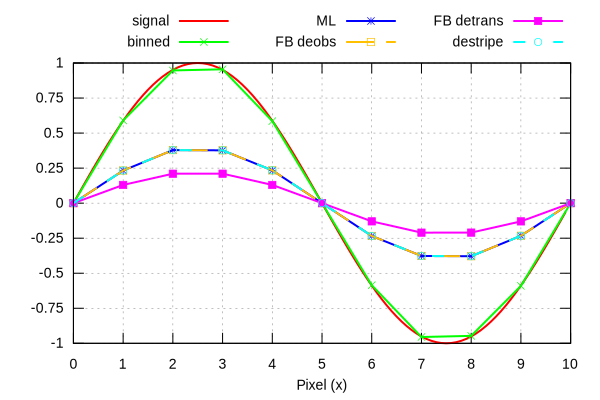
\includegraphics[width=\columnwidth]{subpix/model_error_toy.pdf}
	\caption{
		Demonstration of large loss of power in long-wavelength mode
		caused by the poor subpixel treatment in the standard nearest-neighbor pointing matrix.
		Figure~\ref{fig:ps} shows the noise model/inverse weights/inverse filter
		used in the various methods.
		\dfn{signal}: The input signal, a smooth long-wavelength mode,
		sampled at 10 samples per output pixel.
		\dfn{binned}: Simple binned map (the unweighted average per pixel).
		Very suboptimal in the presence of correlated noise, but unbiased.
		\dfn{ML}: Maximum-likelihood map. 2/3 of the signal is lost despite
		the naive expectation of biaslessness for this estimator.
		\dfn{FB deobs}: Filter+bin map debiased using an observation matrix.
		Identical to ML.
		\dfn{FB detrans}: Filter+bin map debiased by deconvolving a
		transfer function measured from simulations. Even more biased
		than the others due to ignoring mode coupling.
		\dfn{destripe}: Destriper in the limit of 1-sample baselines.
		Identical to ML.
	}
	\label{fig:subpix-bias}
\end{figure}

\begin{figure}
	\centering
	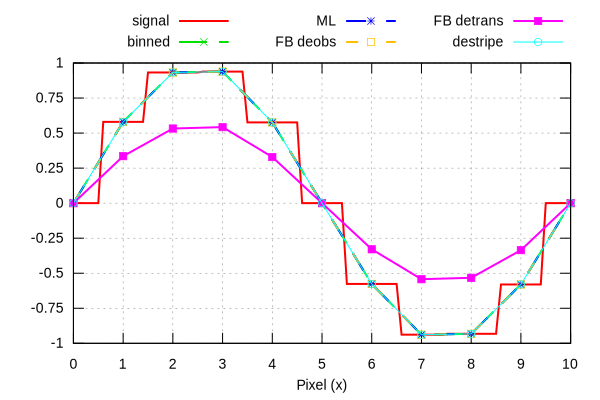
\includegraphics[width=\columnwidth]{subpix/model_error_toy_noerr.pdf}
	\caption{
		Like figure~\ref{fig:subpix-bias}, but with the input signal
		having the same nearest-neighbor pixelization as the models.
		In this case all models except FB detrans are unbiased.
	}
	\label{fig:subpix-noerr}
\end{figure}

\begin{figure}
	\centering
	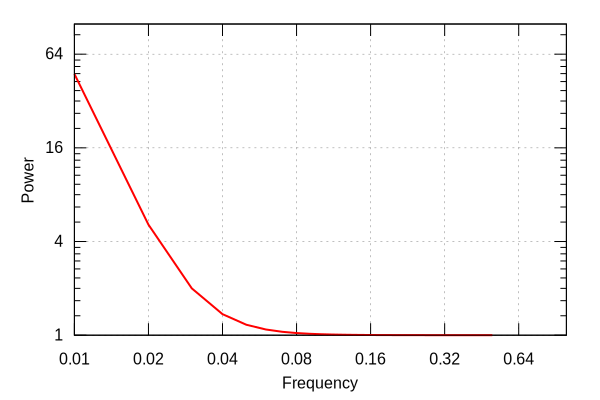
\includegraphics[width=\columnwidth]{subpix/ps.pdf}
	\caption{
		The noise model/inverse weights/inverse filter used in the subpixel
		bias demonstration in figures~\ref{fig:subpix-bias} and \ref{fig:subpix-noerr}.
		It is a simple Fourier-diagonal 1/f + white noise spectrum
		typical for ground-based CMB observations.
	}
	\label{fig:ps}
\end{figure}

\begin{figure}
	\centering
	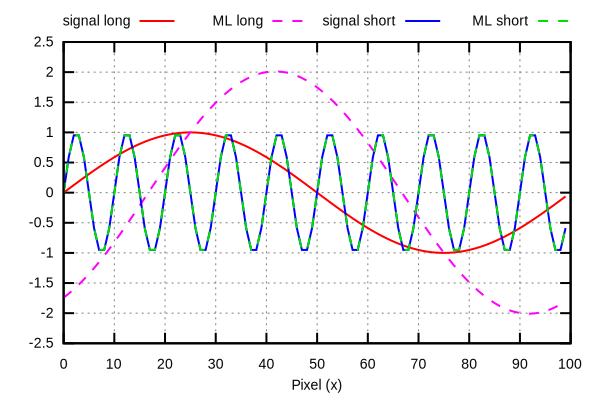
\includegraphics[width=\columnwidth]{common_mode/common.pdf}
	\caption{
		Demonstration of large-scale bias in a multi-detector system
		due to an interaction between strong large-scale
		detector correlations in the noise model and large
		relative gain errors between the detectors.
		\dfn{signal long}: An input long-wavelength signal,
		with the same pixelization as the output to avoid subpixel bias.
		\dfn{ML long}: Corresponding maximum-likelihood map, which
		exhibits both an amplitude and phase error.
		\dfn{signal short} and \dfn{ML short}: The same, but for a
		short-wavelength mode. Here the bias is negligible,
		despite the model's gain errors being scale-independent.
	}
	\label{fig:common}
\end{figure}

\bibliographystyle{act_titles}
\bibliography{refs}

\end{document}
